\documentclass[a4paper,11pt,fleqn]{article}%fleqn pour aligner les equations à gauche
\usepackage{../../Styles/Cours}


\newcommand{\chnum}{Chapitre 16}
\newcommand{\chtitle}{La découverte de l'effet photoélectrique}
\newcommand{\dtype}{Activité}


\begin{document}
\maketitle

%Activité 1 Découverte de l’effet photoélectrique
Au début du 20e siècle, il est solidement établi que la lumière est une onde, bien que quelques observations ne soient pas expliquées. Pour interpréter l’effet photoélectrique, Albert Einstein fait en 1905 l’hypothèse révolutionnaire que la lumière est un flux de particules, mail le monde scientifique n’est pas convaincu. \emph{Comment l’expérience historique de Robert Millikan confirme-t-elle en 1915 l’hypothèse d’Einstein ?}.

\begin{figure}[h!]
	\caption{\textbf{Effet photoélectrique}}
	\label{fig1}
Lorsqu’un métal est exposé à une lumière du domaine ultraviolet ou visible, des électrons peuvent être éjectés du métal grâce à l’énergie lumineuse reçue. On les nomme « photoélectrons ».\\
L’effet photoélectrique ne dépend pas de la puissance du faisceau lumineux. Il se produit dès que le métal est éclairé (pas de délai) à condition que la fréquence $\nu$ du rayonnement soit supérieure à une «\textbf{fréquence seuil}», $\nu_0$, caractéristique du métal. Si $\nu$ est inférieure à $\nu_0$, aucun électron n’est éjecté de la surface du métal, même pour un faisceau lumineux de forte puissance et pour une durée d’éclairement élevée.\\
Ces observations auront une importance capitale dans la compréhension de la nature de la lumière.
\begin{center}
\begin{tikzpicture}[scale=.6, transform shape]
	\shadedraw (0,0)--(3,-2) --(6,0)--(3,2)--cycle;
	\shadedraw (0,0)--(0,-.2) --(3,-2.2) --(3,-2)--cycle;
	\shadedraw (3,-2)--(3,-2.2) --(6,-.2)-- (6,0)--cycle;
	\draw [rotate=-35,domain=-3:2,samples=1000, red, thick] plot (\x,{1.8+.3*sin(200*\x+90)});
	\draw [rotate=-35,domain=-3:2,samples=1000, red, thick] plot (\x,{.8+.3*sin(200*\x+90)});
	\draw [rotate=-35,domain=-3:2,samples=1000, red, thick] plot (\x,{2.8+.3*sin(200*\x+90)});
	\draw [rotate=-35,-Latex,red,very thick] (-.1,1.1) to (0,1.2);
	\draw [rotate=-35,-Latex,red,very thick] (0,2.2) to (.1,2.3);
	\draw [rotate=-35,-Latex,red,very thick] (0.0,3.2) to (.1,3.3);
	\node[fill=red] (nu) at (3.5,5){\Huge \color{white}{$\mathbf{\nu < \nu_0}$}};
\end{tikzpicture}
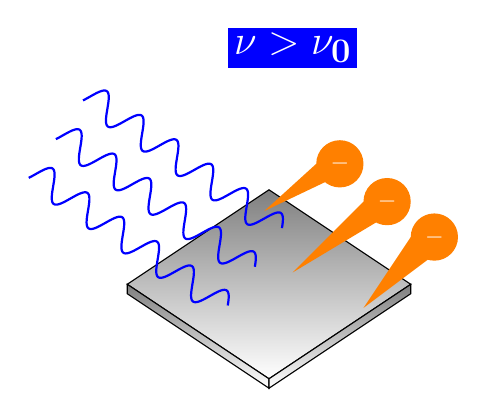
\begin{tikzpicture}[scale=.6, transform shape]
	\shadedraw (0,0)--(3,-2) --(6,0)--(3,2)--cycle;
	\shadedraw (0,0)--(0,-.2) --(3,-2.2) --(3,-2)--cycle;
	\shadedraw (3,-2)--(3,-2.2) --(6,-.2)-- (6,0)--cycle;
	\draw [rotate=-35,domain=-3:2,samples=1000, blue, thick] plot (\x,{1.8+.3*sin(400*\x+90)});
	\draw [rotate=-35,domain=-3:2,samples=1000, blue, thick] plot (\x,{.8+.3*sin(400*\x+90)});
	\draw [rotate=-35,domain=-3:2,samples=1000, blue, thick] plot (\x,{2.8+.3*sin(400*\x+90)});
	
	
	\node[fill=blue] (nu) at (3.5,5){\Huge \color{white}{$\mathbf{\nu > \nu_0}$}};
	
	\fill[fill=orange] (6.5,1) circle(.5);
	\fill[fill=orange] (5.5,1.75) circle(.5);
	\fill[fill=orange] (4.5,2.55) circle(.5);
	
	\fill[fill=orange] (5,-0.5) -- (6,1) -- (7,1)--cycle;
	\fill[fill=orange] (3.5,0.25) -- (5,1.75) -- (6,1.75)--cycle;
	\fill[fill=orange] (2.9,1.55) -- (4,2.55) -- (5,2.55)--cycle;
	
	\node[white] (m1) at (6.5,1){\Large $-$};
	\node[white] (m2) at (5.5,1.75){\Large $-$};
	\node[white] (m3) at (4.5,2.55){\Large $-$};
	
	
\end{tikzpicture}
\end{center}
\end{figure}

\begin{figure}[h!]
	\caption{\textbf{Échec du modèle ondulatoire}}
	\label{fig2}
\begin{multicols}{2} 
 Telle un onde à la surface de l’eau qui transmet de l’énergie à une bouée en la mettant en mouvement, l’énergie d’une onde lumineuse est transmise de manière \textbf{continue}
 à la matière.\\
D’après la conception ondulatoire de la lumière admise au début du 20e siècle, un électron du métal devrait  absorber et accumuler de l’énergie transférée par la lumière, proportionnellement à la puissance lumineuse et à la durée de l’éclairement, jusqu’à être éjecté.\\
En effet, certains des électrons présents dans un métal peuvent s’y déplacer mais sont retenus dans le métal. Pour qu’un électron puisse franchir la surface du métal, il faut fournir au système \{électron/métal\} une énergie minimale $\mathcal{W}_e$, appelée « \textbf{travail d’extraction}» au métal.\\
\columnbreak
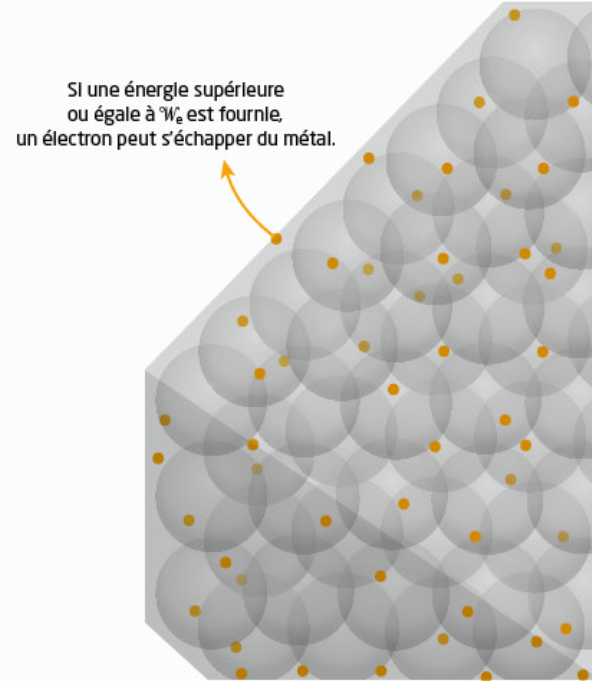
\includegraphics[width=.8\linewidth]{Ressources/TSPE_C16_Act1_fig1.png}
\end{multicols}
\end{figure}

 
\begin{figure}[h!]
	\caption{\textbf{Hypothèse d’Einstein}}
	\label{fig3}
\begin{multicols}{2}
\begin{wrapfigure}{l}{0.15\textwidth}
    \centering
    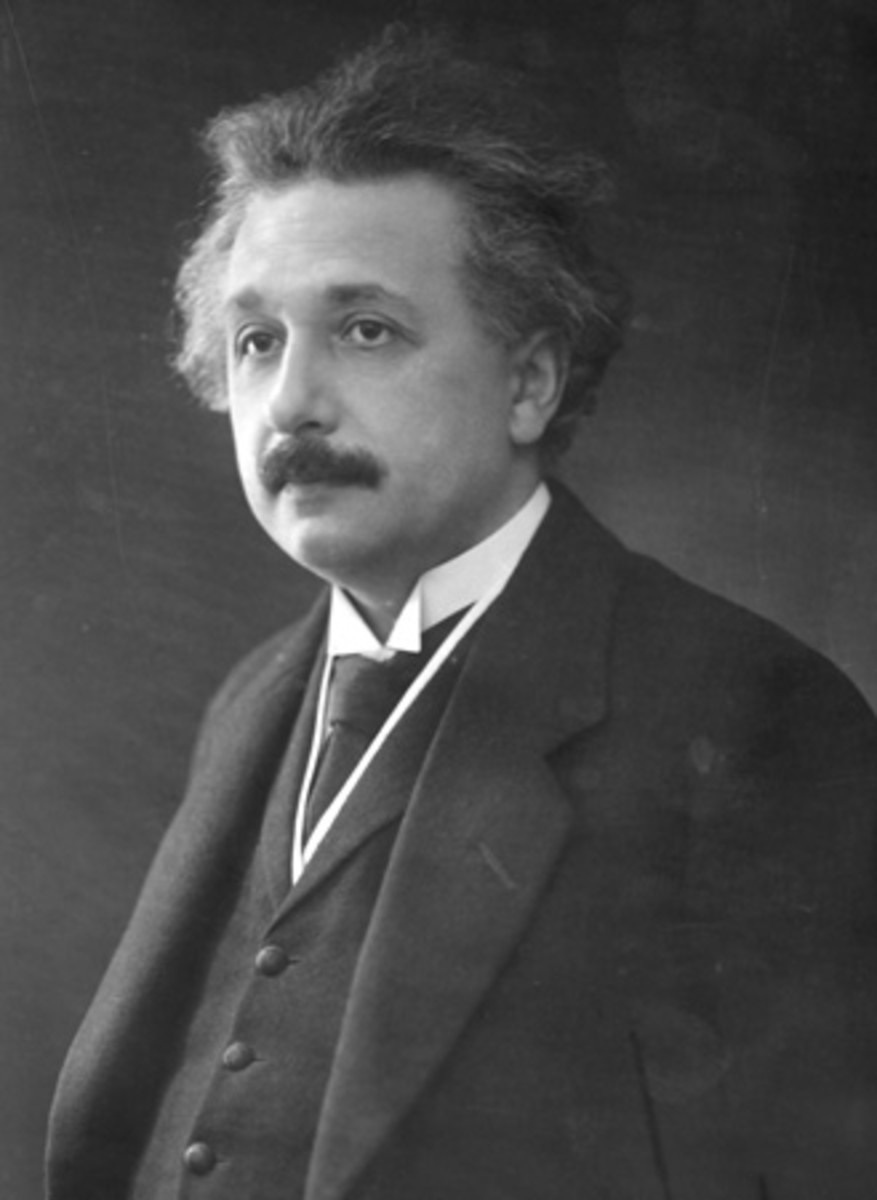
\includegraphics[width=0.15\textwidth]{Ressources/TSPE_C16_Act1_Einstein.jpg}
\end{wrapfigure}
En 1905, Albert Einstein suppose que la lumière est constituée de \textbf{quanta}, plus tard nommés \textbf{photons}. Pour que l’effet photoélectrique se produise, l’énergie d’un photon incident doit au moins être égale au travail d’extraction. Dans ce cas le photon est absorbé, il transfert la totalité de son énergie, et un seul électron est éjecté.\\
\emph{Lorsque l’énergie du photon incident est supérieure au travail d’extraction, l’excès d’énergie est transférée sous forme d’énergie cinétique à l’électron émis.}
\columnbreak

\begin{wrapfigure}{r}{0.15\textwidth}
    \centering
    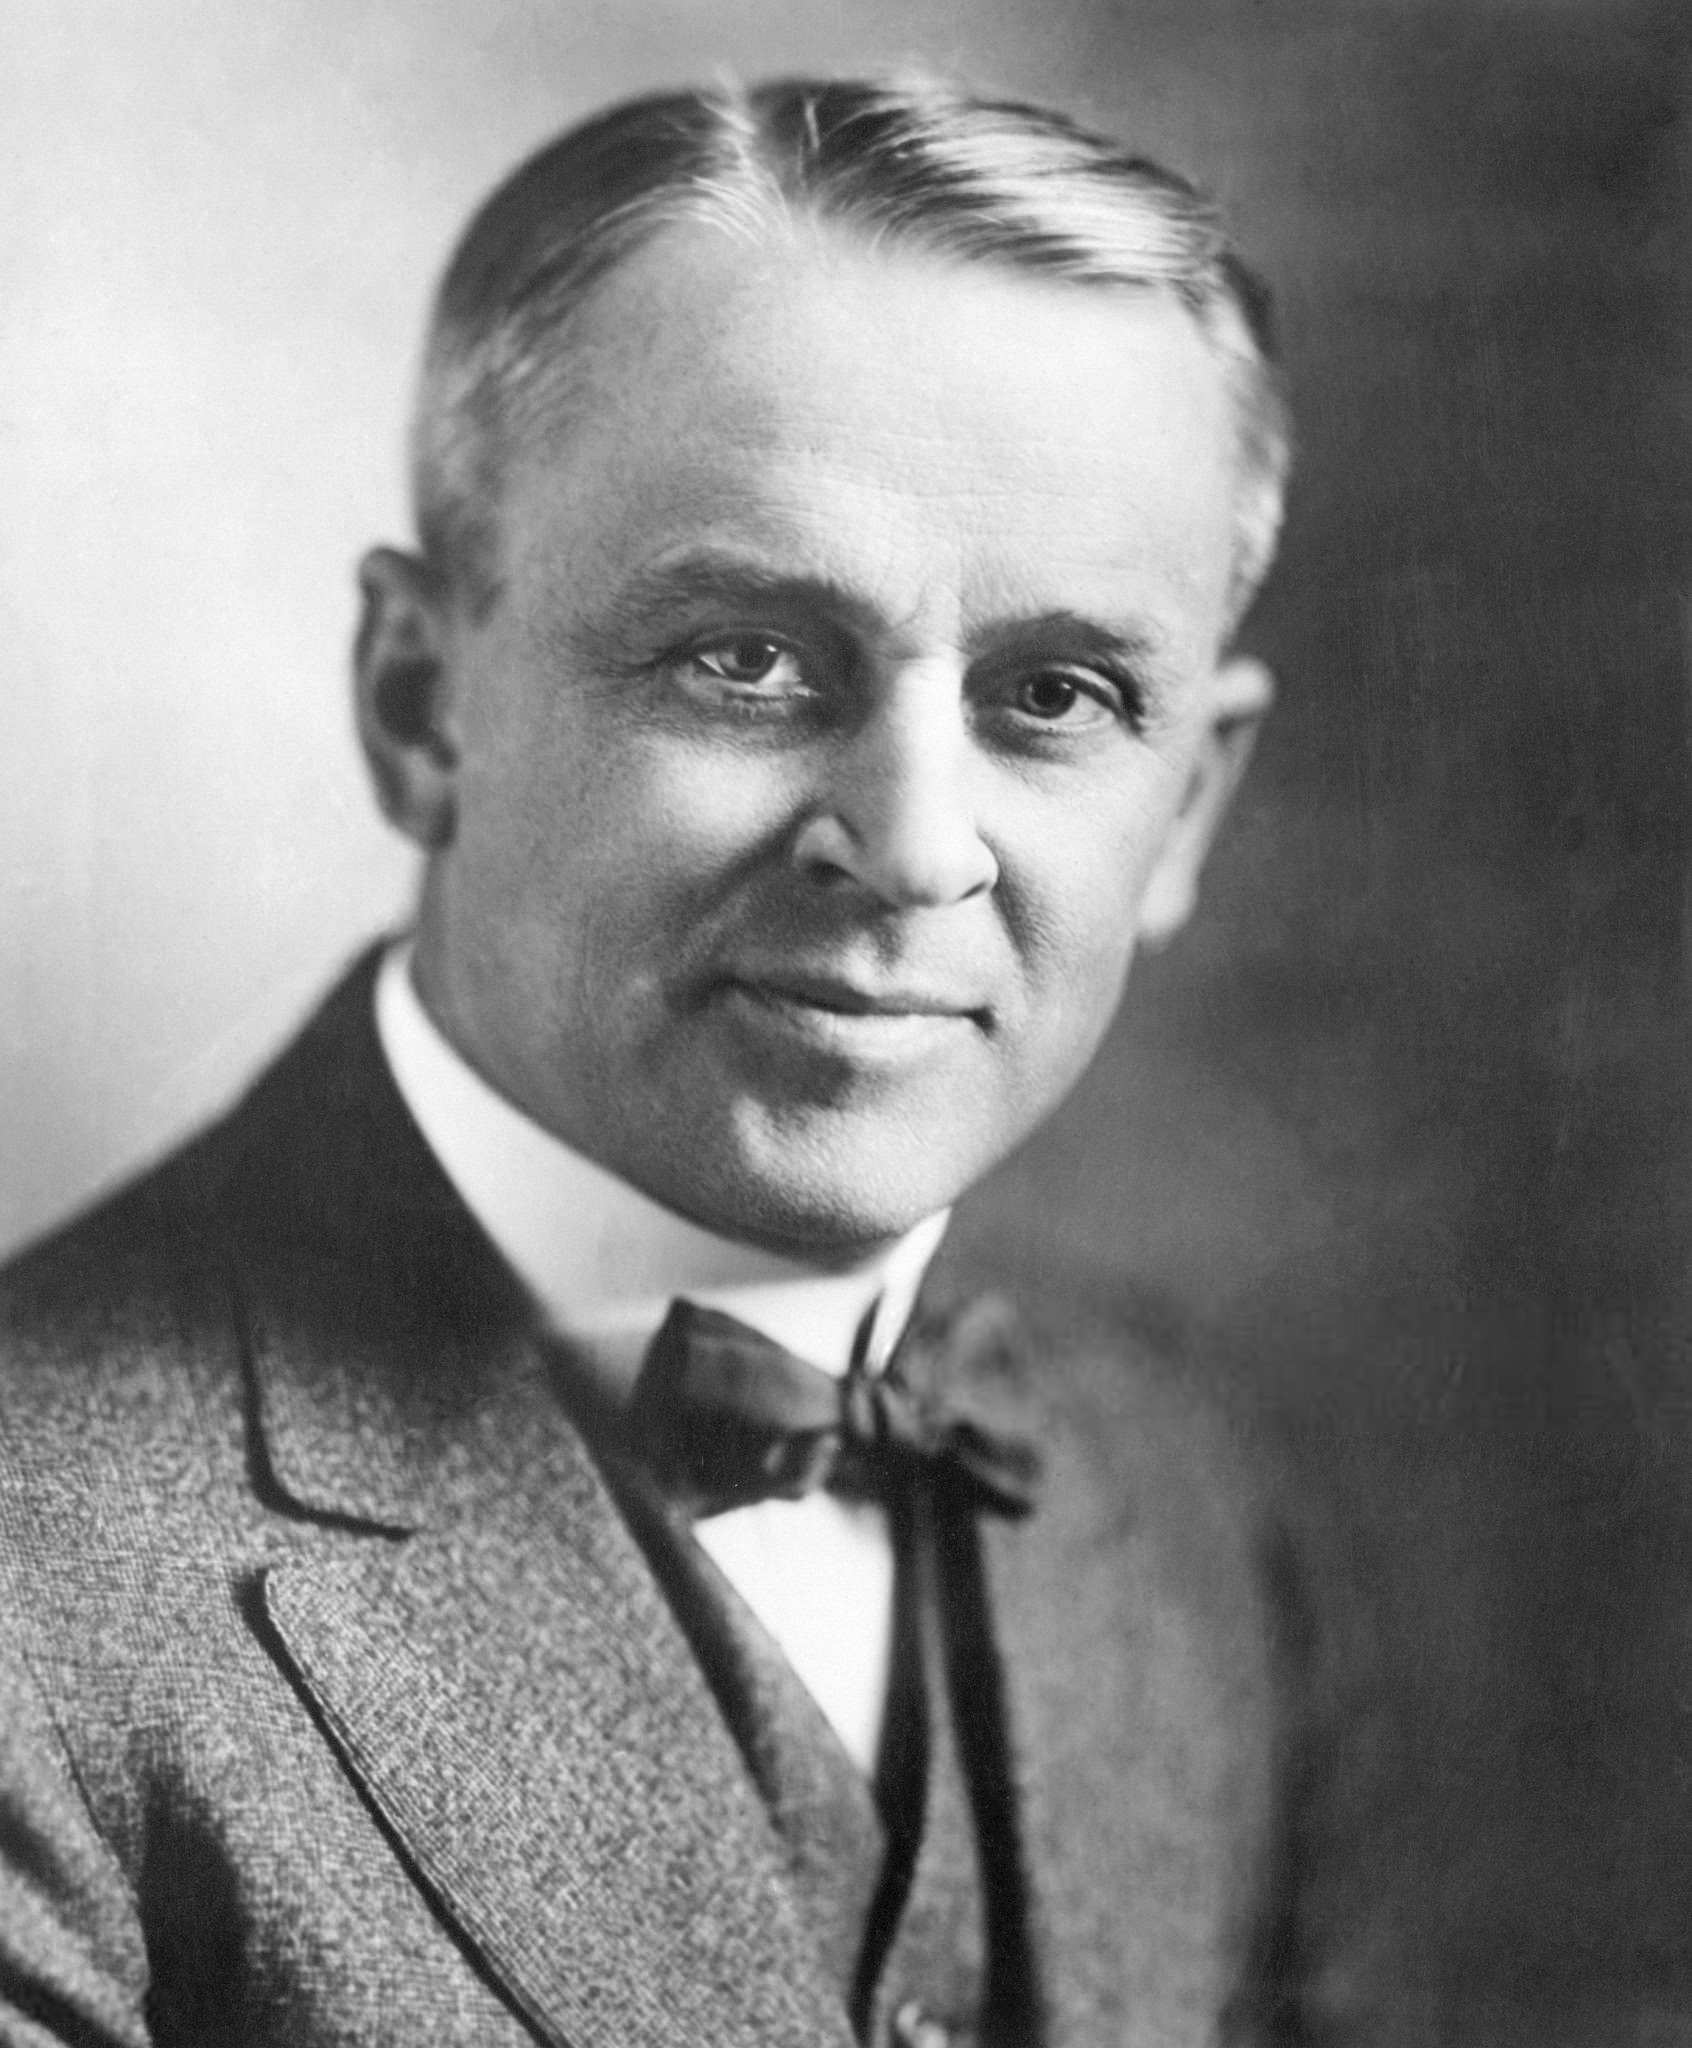
\includegraphics[width=0.15\textwidth]{Ressources/TSPE_C16_Act1_Millikan.jpg}
\end{wrapfigure}
Dans son autobiographie, Robert Millikan écrit : «J’ai passé dix ans de ma vie à vérifier expérimentalement l’équation trouvée par Einstein en 1905, et contrairement à toutes mes prévisions, je fus contraint, en 1915, d’affirmer que sa confirmation était indiscutable en dépit de son caractère déraisonnable, car elle semblait contredire tout ce que nous savions sur les interférences lumineuses.».
\end{multicols}
\end{figure}

\begin{figure}[h!]
	\caption{\textbf{Schéma du principe de l’expérience de Millikan et résultats (1915)}}
	\begin{multicols}{2}
La mesure de l’intensité $I$ du courant électrique permet d’estimer le nombre d’électrons émis par la cathode lorsqu’elle est éclairée. L’énergie cinétique maximale $\mathcal{E}_{c,max}$ des électrons est déterminée en mesurant la tension $U_{PN}$ au-delà de laquelle aucun courant électrique ne passe plus.
\begin{center}
	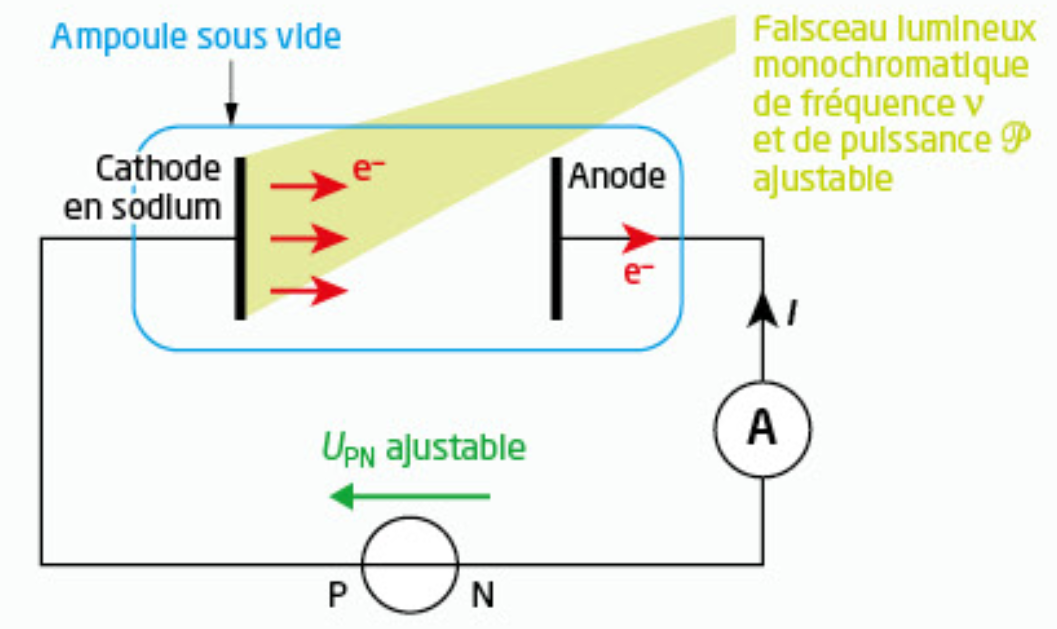
\includegraphics[width=.7\linewidth]{Ressources/TSPE_C16_Act1_fig4a.png}
\end{center}
\columnbreak
Pour une fréquence donnée, on observe qu’il n’y a qu’une seule valeur de $\mathcal{E}_{c,max}$, quelle que soit la puissance $\mathcal{P}$ du faisceau lumineux.
\begin{center}
	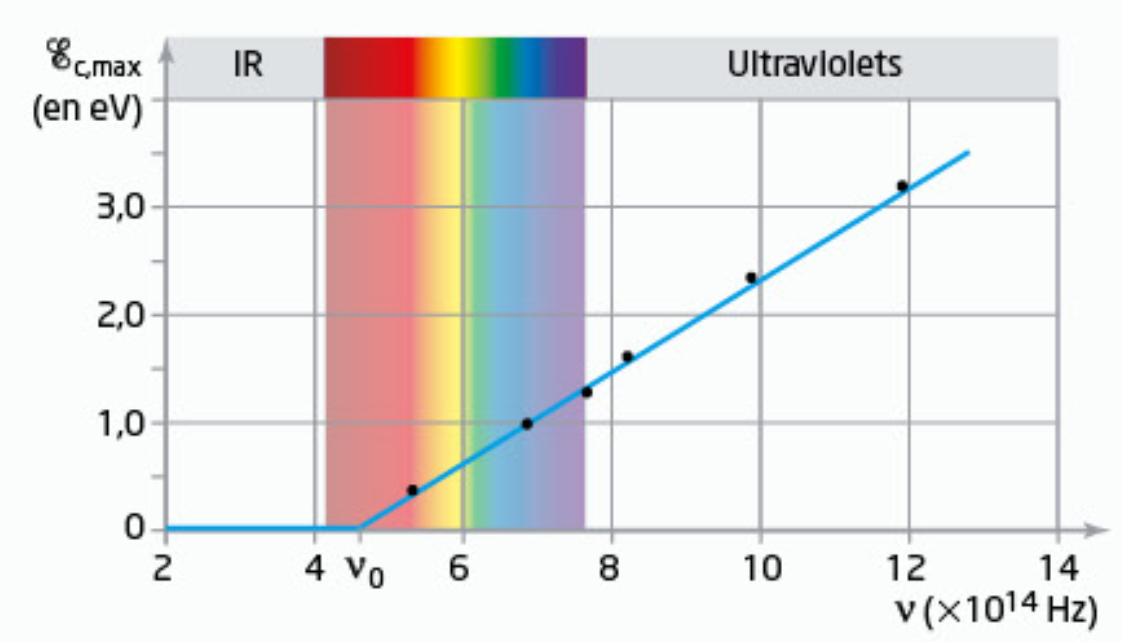
\includegraphics[width=.9\linewidth]{Ressources/TSPE_C16_Act1_fig4b.png}
\end{center}
\end{multicols}
\label{fig4}
\end{figure}

\noindent \colorbox{blue!10}{
\begin{minipage}{\linewidth}
\centering  \textcolor{purple!50!blue!70}{\Large \textbf{Questions}}
\begin{multicols}{2}
\begin{enumerate}
	\item S’approprier
	\begin{enumerate}
		\item Présenter l’effet photoélectrique et indiquer pour quel type de lumière il se manifeste.
		\item Rappeler l’hypothèse d’Einstein concernant l’expression d’un quantum d’énergie transportée par la lumière.
	\end{enumerate}
	\item Analyser - Raisonner
	\begin{enumerate}
		\item Expliquer en quoi les conditions d’observation de l’effet photoélectrique (Doc.~\ref{fig1}) sont en contradiction avec une description purement ondulatoire de la lumière (Doc.~\ref{fig2}).
		\item Expliquer en quoi la notion de photon permet d’interpréter l’existence de la fréquence seuil.
	\end{enumerate}
	\item Réaliser\\
	En s’inspirant de la phrase surlignée dans le Doc.~\ref{fig3}, établir, par un bilan d’énergie, la relation entre l’énergie cinétique maximale $\mathcal{E}_{c,max}$ des photoélectrons lorsqu’ils sont émis et la fréquence $\nu$ de la lumière.
	\item Valider
	\begin{enumerate}
		\item Montrer qualitativement que la relation précédente est vérifiée par les mesures du Doc.~\ref{fig4} en justifiant l’allure de la représentation graphique pour $\nu >\nu_0$.
		\item En utilisant les documents, dégager l’importance historique de l’effet photoélectrique.
	\end{enumerate}

\end{enumerate}
\end{multicols}
\end{minipage}
}
 

\end{document}